% Options for packages loaded elsewhere
\PassOptionsToPackage{unicode}{hyperref}
\PassOptionsToPackage{hyphens}{url}
%
\documentclass[
  ignorenonframetext,
  aspectratio=169,
]{beamer}
\usepackage{pgfpages}
\setbeamertemplate{caption}[numbered]
\setbeamertemplate{caption label separator}{: }
\setbeamertemplate{navigation symbols}{}
\setbeamertemplate{footline}[page number]
\setbeamertemplate{itemize item}{\small\raise0.5pt\hbox{$\bullet$}}
\setbeamertemplate{itemize subitem}{\tiny\raise1.5pt\hbox{$\bullet$}}
\setbeamertemplate{itemize subsubitem}{\tiny\raise1.5pt\hbox{$\bullet$}}
\setbeamercolor{caption name}{fg=normal text.fg}
\beamertemplatenavigationsymbolsempty
% Prevent slide breaks in the middle of a paragraph
\widowpenalties 1 10000
\raggedbottom
\setbeamertemplate{part page}{
  \centering
  \begin{beamercolorbox}[sep=16pt,center]{part title}
    \usebeamerfont{part title}\insertpart\par
  \end{beamercolorbox}
}
\setbeamertemplate{section page}{
  \centering
  \begin{beamercolorbox}[sep=12pt,center]{part title}
    \usebeamerfont{section title}\insertsection\par
  \end{beamercolorbox}
}
\setbeamertemplate{subsection page}{
  \centering
  \begin{beamercolorbox}[sep=8pt,center]{part title}
    \usebeamerfont{subsection title}\insertsubsection\par
  \end{beamercolorbox}
}
\AtBeginPart{
  \frame{\partpage}
}
\AtBeginSection{
  \ifbibliography
  \else
    \frame{\sectionpage}
  \fi
}
\AtBeginSubsection{
  \frame{\subsectionpage}
}
\usepackage{amsmath,amssymb}
\usepackage{lmodern}
\usepackage{iftex}
\ifPDFTeX
  \usepackage[T1]{fontenc}
  \usepackage[utf8]{inputenc}
  \usepackage{textcomp} % provide euro and other symbols
\else % if luatex or xetex
  \ifXeTeX
    \usepackage{xltxtra} 
    \usepackage{xeCJK}
    \setCJKmainfont{ipaexm.ttf}
    \setCJKsansfont{ipaexg.ttf}
    \setCJKmonofont{ipaexg.ttf}
  \fi
  \usepackage{unicode-math}
  \defaultfontfeatures{Scale=MatchLowercase}
  \defaultfontfeatures[\rmfamily]{Ligatures=TeX,Scale=1}
\fi
% Use upquote if available, for straight quotes in verbatim environments
\IfFileExists{upquote.sty}{\usepackage{upquote}}{}
\IfFileExists{microtype.sty}{% use microtype if available
  \usepackage[]{microtype}
  \UseMicrotypeSet[protrusion]{basicmath} % disable protrusion for tt fonts
}{}
\makeatletter
\@ifundefined{KOMAClassName}{% if non-KOMA class
  \IfFileExists{parskip.sty}{%
    \usepackage{parskip}
  }{% else
    \setlength{\parindent}{0pt}
    \setlength{\parskip}{6pt plus 2pt minus 1pt}}
}{% if KOMA class
  \KOMAoptions{parskip=half}}
\makeatother
\usepackage{xcolor}
\IfFileExists{xurl.sty}{\usepackage{xurl}}{} % add URL line breaks if available
\IfFileExists{bookmark.sty}{\usepackage{bookmark}}{\usepackage{hyperref}}
\hypersetup{
  pdftitle={Estimating Effect of Tax Incentives on Charitable Giving Considering Self-Selection of Tax Relief in South Korea},
  hidelinks,
  pdfcreator={LaTeX via pandoc}}
\urlstyle{same} % disable monospaced font for URLs

\usepackage{setspace}
\usepackage{float}

\newif\ifbibliography
\usepackage{longtable,booktabs,array}
\usepackage{threeparttable, threeparttablex, multirow}
\usepackage{calc} % for calculating minipage widths
\usepackage{caption}
% Make caption package work with longtable
\makeatletter
\def\fnum@table{\tablename~\thetable}
\makeatother
\usepackage{graphicx}
\makeatletter
\def\maxwidth{\ifdim\Gin@nat@width>\linewidth\linewidth\else\Gin@nat@width\fi}
\def\maxheight{\ifdim\Gin@nat@height>\textheight\textheight\else\Gin@nat@height\fi}
\makeatother
% Scale images if necessary, so that they will not overflow the page
% margins by default, and it is still possible to overwrite the defaults
% using explicit options in \includegraphics[width, height, ...]{}
\setkeys{Gin}{width=\maxwidth,height=\maxheight,keepaspectratio}
% Set default figure placement to htbp
\makeatletter
\def\fps@figure{htbp}
\makeatother
\setlength{\emergencystretch}{3em} % prevent overfull lines
\providecommand{\tightlist}{%
  \setlength{\itemsep}{0pt}\setlength{\parskip}{0pt}}
\setcounter{secnumdepth}{-\maxdimen} % remove section numbering
\newlength{\cslhangindent}
\setlength{\cslhangindent}{1.5em}
\newlength{\csllabelwidth}
\setlength{\csllabelwidth}{3em}
\newlength{\cslentryspacingunit} % times entry-spacing
\setlength{\cslentryspacingunit}{\parskip}
\newenvironment{CSLReferences}[2] % #1 hanging-ident, #2 entry spacing
 {% don't indent paragraphs
  \setlength{\parindent}{0pt}
  % turn on hanging indent if param 1 is 1
  \ifodd #1
  \let\oldpar\par
  \def\par{\hangindent=\cslhangindent\oldpar}
  \fi
  % set entry spacing
  \setlength{\parskip}{#2\cslentryspacingunit}
 }%
 {}
\usepackage{calc}
\newcommand{\CSLBlock}[1]{#1\hfill\break}
\newcommand{\CSLLeftMargin}[1]{\parbox[t]{\csllabelwidth}{#1}}
\newcommand{\CSLRightInline}[1]{\parbox[t]{\linewidth - \csllabelwidth}{#1}\break}
\newcommand{\CSLIndent}[1]{\hspace{\cslhangindent}#1}


\ifLuaTeX
  \usepackage{selnolig}  % disable illegal ligatures
\fi

\title{Estimating Effect of Tax Incentives on Charitable Giving Considering Self-Selection of Tax Relief in South Korea  }
\author[shortname]{ Hiroki Kato \inst{1} \and  Tsuyoshi Goto \inst{2} \and  Yong-Rok Kim \inst{3} \and }
\institute[shortinst]{ \inst{1} Osaka University \and  \inst{2} Chiba University \and  \inst{3} Kansai University \and }

\date{2021/12/18}


\begin{document}
\frame{\titlepage}

\begin{frame}{Introduction}
\protect\hypertarget{introduction}{}
\begin{itemize}
\tightlist
\item
  In many countries, tax relief for charitable giving are implemented.
\item
  The elasticity of giving tax relief is known as a key parameter to evaluate the welfare implication (Saez, 2004).

  \begin{itemize}
  \tightlist
  \item
    Intuitively, if the elasticity is more than 1 in absolute value, \$1 of tax relief make more than \$1 of charitable giving.
  \end{itemize}
\item
  Many papers investigate the elasticity based on tax return data (Almunia et al., 2020; Auten et al., 2002).
\end{itemize}
\end{frame}

\begin{frame}{Introduction}
\protect\hypertarget{introduction-1}{}
\begin{itemize}
\tightlist
\item
  However, the tax return data record only the declared charitable giving.

  \begin{itemize}
  \tightlist
  \item
    First issue: \textbf{Actual donations is different from declared donations.} (Fack and Landais, 2016; Gillitzer and Skov, 2018)
  \item
    We use panel survey data in South Korea to deal with this issue.
  \end{itemize}
\item
  Tax payers decide the amount of donation and whether to declare tax relief based on the size of tax incentive and declaration cost.

  \begin{itemize}
  \tightlist
  \item
    Second issue: Neglect of this declaration cost may bias the estimations of elasticity.
  \item
    We use instrumental variable (IV) and control function approach for this issue.
  \end{itemize}
\item
  Based on DID as an identification strategy, we investigate the giving price elasticity of South Korea.
\end{itemize}
\end{frame}

\begin{frame}{Introduction}
\protect\hypertarget{introduction-2}{}
Result

\begin{enumerate}
\tightlist
\item
  Baseline results show that the giving price elasticity is less than -1.4 in terms of intensive margins and less than -1.7 in terms of extensive margins in Korea.
\item
  The estimated giving price elasticity for those who declare charitable giving is around -1.2 -1.6.

  \begin{itemize}
  \tightlist
  \item
    These estimates are more elastic than the estimates in the extant research, many of which show around -1.
  \end{itemize}
\item
  By reducing application cost, we can increase charitable giving.
\item
  Given our estimates, increasing the subsidy on charitable giving will be desirable in Korea.
\end{enumerate}
\end{frame}

\hypertarget{conceptual-framework}{%
\section{Conceptual Framework}\label{conceptual-framework}}

\begin{frame}{Optimization Problem}
\protect\hypertarget{optimization-problem}{}
Following Almunia et al. (2020),
consider allocation problem between private consumption (\(x_{it}\)) and charitable giving (\(g_{it}\))

\begin{align}
  \max_{x_{it}, g_{it}, R_{it}} &U(x_{it}, g_{it}, G_t)
  = u_i(x_{it}, g_{it}, G_t) - R_{it}K(Z_{it}), \\
  \text{s.t.}\:\:
  &x_{it} + g_{it}
  = y_{it} - R_{it} T_{it}(y_{it}, g_{it}) - (1 - R_{it}) T_{it}(y_{it}), \\
  &G_t = g_{it} + G_{-it},
\end{align}

where \(y_{it}\) is pre-tax total income, \(R_{it}\) is a dummy of declaration of tax relief and \(T_{it}(y_{it})\) and \(T_{it}(y_{it}, g_{it})\) are respectively the amount of tax when \(i\) does not declare tax relief and when \(i\) declares tax relief in year \(t\). \(G_{-it}\) is public goods supplied by others. \(K(Z_{it})\) is application cost which is a function of instrument \(Z_{it}\).
\end{frame}

\begin{frame}{Remarks on Optimization Problem}
\protect\hypertarget{remarks-on-optimization-problem}{}
We assume

\begin{itemize}
\tightlist
\item
  No saving
\item
  \(G_{-it}\) is large enough to \(\frac{\partial u_i}{\partial G}(x, g, G) \approx 0\)
\end{itemize}

Given \(R_{it}\), optimal level of donations sloves

\begin{align}
  \max_{g_{it}} u_i(
    y_{it} - R_{it} T_{it}(y_{it}, g_{it}) - (1 - R_{it}) T_{it}(y_{it}) - g_{it}, g_{it}, g_{it} + G_{-it}
  ).
\end{align}

\begin{itemize}
\tightlist
\item
  We can ignore application cost \(K(Z_{it})\) when solving optimal giving level because the application cost does not depend on \(g_{it}\)
\end{itemize}
\end{frame}

\begin{frame}{First-Order Condition}
\protect\hypertarget{first-order-condition}{}
\begin{align}
  - \frac{\partial u_i}{\partial x_{it}}
  \left( R_{it} \frac{\partial T_{it}}{\partial g_{it}}(y_{it}, g_{it}) + 1 \right)
  + \frac{\partial u_i}{\partial g_{it}} = 0
\end{align}

\begin{itemize}
\tightlist
\item
  \(\partial T_{it} / \partial g_{it} < 0\) is tax incentive of charitable giving.

  \begin{itemize}
  \tightlist
  \item
    Let \(s_{it} \equiv |\partial T_{it} / \partial g_{it}|\) be size of tax incentive.
  \item
    Relative giving price is \(1 - s_{it}\)
  \item
    As we explain later, there is \emph{within} variation of \(s_{it}\) due to tax reform.
  \end{itemize}
\end{itemize}

Define \(g_i(1 - s_{it}, y_{it})\) and \(g_i(1, y_{it})\) to be the optimal levels of donations (potential outcomes) for choices \(R_{it} = 1, 0\) respectively.
\end{frame}

\begin{frame}{Self-Selection of Tax Relief}
\protect\hypertarget{self-selection-of-tax-relief}{}
We can write indirect utility as

\begin{align}
  &v_i(1 - s_{it}, y_{it}, G_{-it}) - K(Z_{it}),  \\
  &v_i(1, y_{it}, G_{-it}).
\end{align}

Thus, individual \(i\) applies for tax relief in year \(t\),
that is, \(R_{it} = 1\) iff

\begin{align}
  \Delta v_{it} \equiv
  v_i(1 - s_{it}, y_{it}, G_{-it}) - v_i(1, y_{it}, G_{-it})
  \ge K(Z_{it}).
\end{align}
\end{frame}

\hypertarget{institutional-background-in-south-korea}{%
\section{Institutional Background in South Korea}\label{institutional-background-in-south-korea}}

\begin{frame}{2014 Tax Reform}
\protect\hypertarget{tax-reform}{}
Since 2014, tax relief of charitable giving has changed from \textbf{income deduction (所得控除)} to \textbf{tax credit (税額控除)}.

\begin{itemize}
\tightlist
\item
  Income deductions are more advantageous for high-income groups than low-income groups because the higher the income, the greater the decrease in tax burden.
\item
  The 2014 tax reform aimed to alleviate the regressiveness of taxes and improve the equilibrium of taxation by changing from income deductions to tax credits.
\item
  We exploit this reform as a main source of variation for identification

  \begin{itemize}
  \tightlist
  \item
    Difference-in-Difference
  \end{itemize}
\end{itemize}
\end{frame}

\begin{frame}{2014 Tax Reform}
\protect\hypertarget{tax-reform-1}{}
\textbf{Tax deduction system (until 2013)}

\begin{align}
  T_{it}(y_{it}, g_{it}) = T_{it}(y_{it} - g_{it})
\end{align}

\begin{itemize}
\tightlist
\item
  Tax incentive is \(s_{it} = T'(y_{it} - g_{it})\)
\item
  In 2012 and 2013, the marginal tax rate was the same, though it was different from ones before 2011.
\item
  The giving price depended on income level (\(y_{it}\)) and giving level (\(g_{it}\))
\end{itemize}

\textbf{Tax credit system (from 2014)}

\begin{align}
  T_{it}(y_{it}, g_{it}) = T_{it}(y_{it}) - m g_{it}
\end{align}

\begin{itemize}
\tightlist
\item
  \(m\) is tax credit rate and is \(m = 0.15\)
\item
  Tax incentive is \(s_{it} = m\)
\end{itemize}
\end{frame}

\hypertarget{data}{%
\section{Data}\label{data}}

\begin{frame}{Data}
\protect\hypertarget{data-1}{}
We use the Korean annual financial panel survey,
called the National Survey of Tax and Benefit (hereafter, NaSTaB).

\begin{itemize}
\tightlist
\item
  The subjects of this survey are general households and household members living in 15 cities and provinces nationwide.
\item
  This survey is based on a face-to-face interview.
\item
  Data is constructed as the subjects represent the population of Korean society.
\item
  We exclude the subject of the sample, whose age is under 23, since they are not likely to have income or assets.
\item
  We use data from 2013 to 2017 to focus the 2014 tax reform.
\end{itemize}
\end{frame}

\begin{frame}{Descriptive Statistics}
\protect\hypertarget{descriptive-statistics}{}
\begin{table}

\caption{\label{tab:SummaryCovariate}Descriptive Statistics}
\centering
\fontsize{6}{8}\selectfont
\begin{tabular}[t]{lcccccc}
\toprule
  & N & Mean & Std.Dev. & Min & Median & Max\\
\midrule
\addlinespace[0.3em]
\multicolumn{7}{l}{\textbf{Charitable Donations}}\\
\hspace{1em}Annual chariatable giving (unit: 10,000KRW) & 36259 & 35.86 & 153.36 & 0.00 & 0.00 & 10000.00\\
\hspace{1em}Dummary of donation > 0 & 36259 & 0.24 & 0.43 & 0.00 & 0.00 & 1.00\\
\addlinespace[0.3em]
\multicolumn{7}{l}{\textbf{Income, giving price, and tax report}}\\
\hspace{1em}Annual taxable labor income (unit: 10,000KRW) & 36249 & 1754.32 & 2702.16 & 0.00 & 0.00 & 50000.00\\
\hspace{1em}First giving relative price & 36258 & 0.86 & 0.04 & 0.62 & 0.85 & 0.94\\
\hspace{1em}Dummy of declaration of a tax relief & 36259 & 0.10 & 0.30 & 0.00 & 0.00 & 1.00\\
\addlinespace[0.3em]
\multicolumn{7}{l}{\textbf{Individual Characteristics}}\\
\hspace{1em}Age & 36259 & 53.43 & 16.21 & 24.00 & 51.00 & 103.00\\
\hspace{1em}Female dummy & 36259 & 0.43 & 0.50 & 0.00 & 0.00 & 1.00\\
\hspace{1em}University graduate & 36258 & 0.42 & 0.49 & 0.00 & 0.00 & 1.00\\
\hspace{1em}High school graduate dummy & 36258 & 0.31 & 0.46 & 0.00 & 0.00 & 1.00\\
\hspace{1em}Junior high school graduate dummy & 36258 & 0.27 & 0.44 & 0.00 & 0.00 & 1.00\\
\hspace{1em}Wage earner dummy & 27453 & 0.56 & 0.50 & 0.00 & 1.00 & 1.00\\
\hspace{1em}\#.Tax accountant / population & 36259 & 1.04 & 0.51 & 0.32 & 0.92 & 2.24\\
\bottomrule
\end{tabular}
\end{table}
\end{frame}

\begin{frame}{Income Distribution and Giving Price}
\protect\hypertarget{income-distribution-and-giving-price}{}
\begin{figure}[t]

{\centering 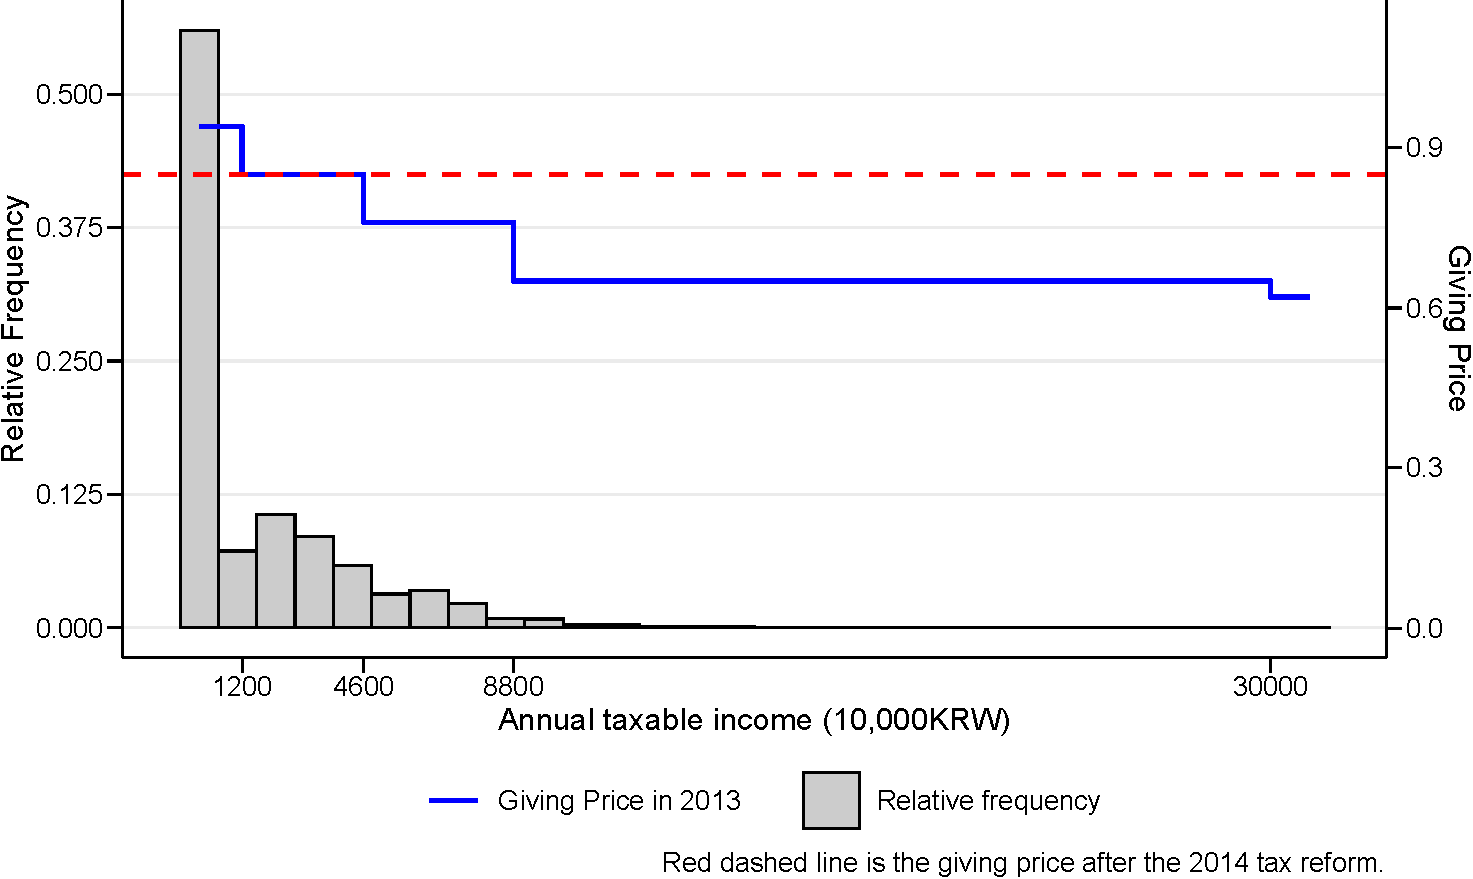
\includegraphics[width=0.7\linewidth,]{C:/Users/katoo/Desktop/NASTAB/paper/slide_files/figure-beamer/SummaryPrice-1} 

}

\caption{Income Distribution and Relative Giving Price in 2013. Notes: The left and right axis measure the relative frequency of respondents and the relative giving price, respectively. A blue step line and a red dashed horizontal line represents the giving price in 2013 and 2014, respectively. The grey bar shows income distribution in 2013.}\label{fig:SummaryPrice}
\end{figure}
\end{frame}

\begin{frame}{Remarks on Figure \ref{fig:SummaryPrice}}
\protect\hypertarget{remarks-on-figure-reffigsummaryprice}{}
The 2014 tax reform

\begin{itemize}
\tightlist
\item
  has decreased the relative price of giving for those whose income is less than 12 million KRW (treatment)
\item
  has unchanged the relative price of giving for those whose income is between 12 million KRW and 46 million KRW (control)
\item
  has increased the relative price of giving for those whose income is more than 46 million KRW (treatment)
\end{itemize}

We exploit this within variation due to exogenous tax reform
for identification.
\end{frame}

\begin{frame}{Charitable Giving By Income Groups}
\protect\hypertarget{charitable-giving-by-income-groups}{}
\begin{figure}[t]

{\centering 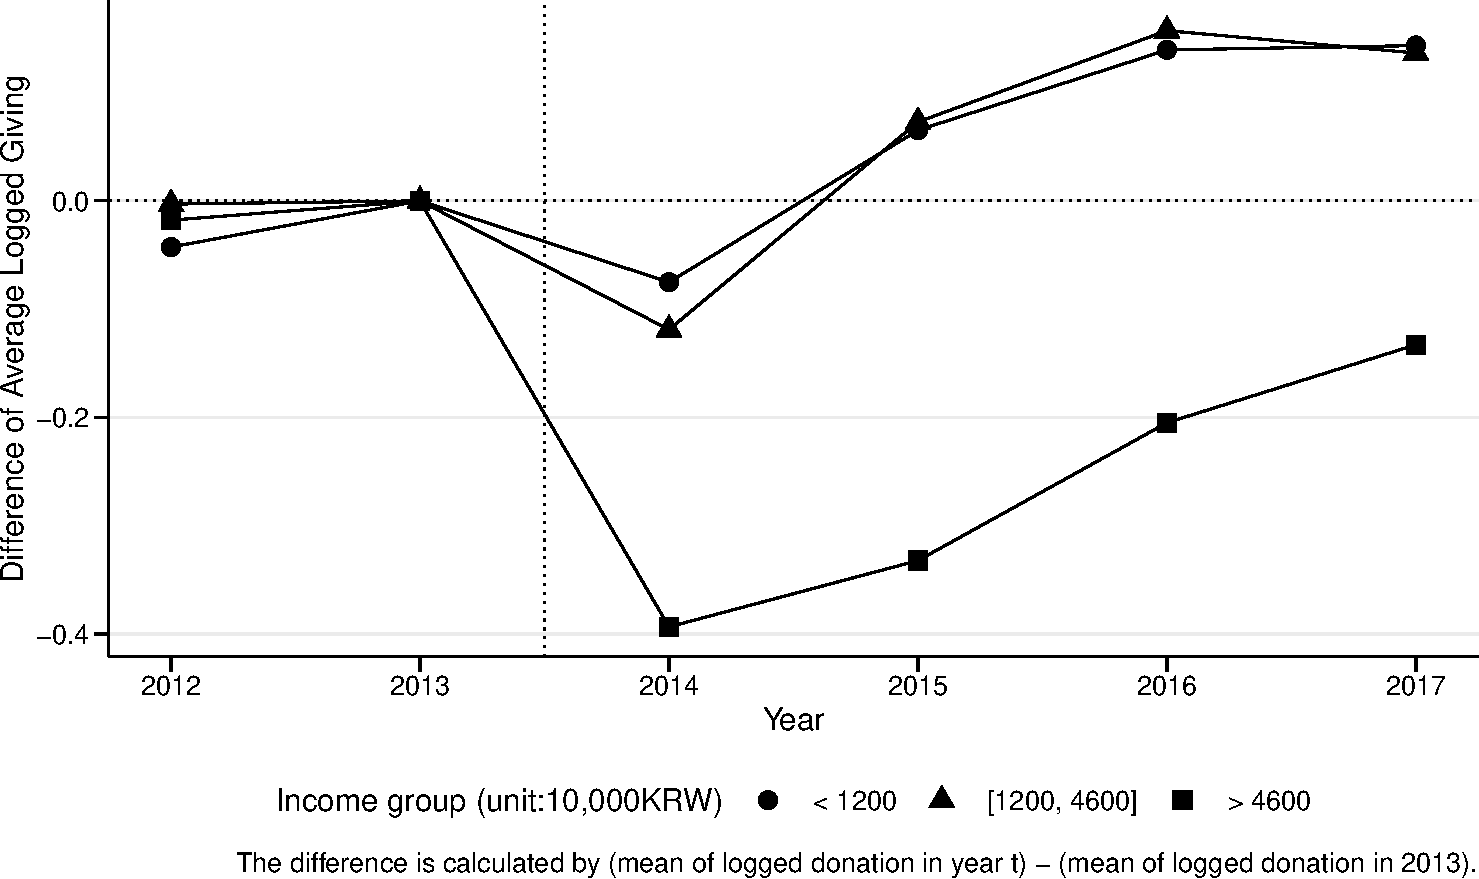
\includegraphics[width=0.7\linewidth,]{C:/Users/katoo/Desktop/NASTAB/paper/slide_files/figure-beamer/SummaryOutcomeOverall-1} 

}

\caption{Average Logged Giving by Three Income Groups. Notes: We created three income groups, with the relative price of giving rising (circle), unchanged (triangle), and falling (square) between 2013 and 2014. The grup means are normalized to be one in 2013.}\label{fig:SummaryOutcomeOverall}
\end{figure}
\end{frame}

\begin{frame}{Charitable Giving by Income Group Conditional On Donors}
\protect\hypertarget{charitable-giving-by-income-group-conditional-on-donors}{}
\begin{figure}[t]

{\centering 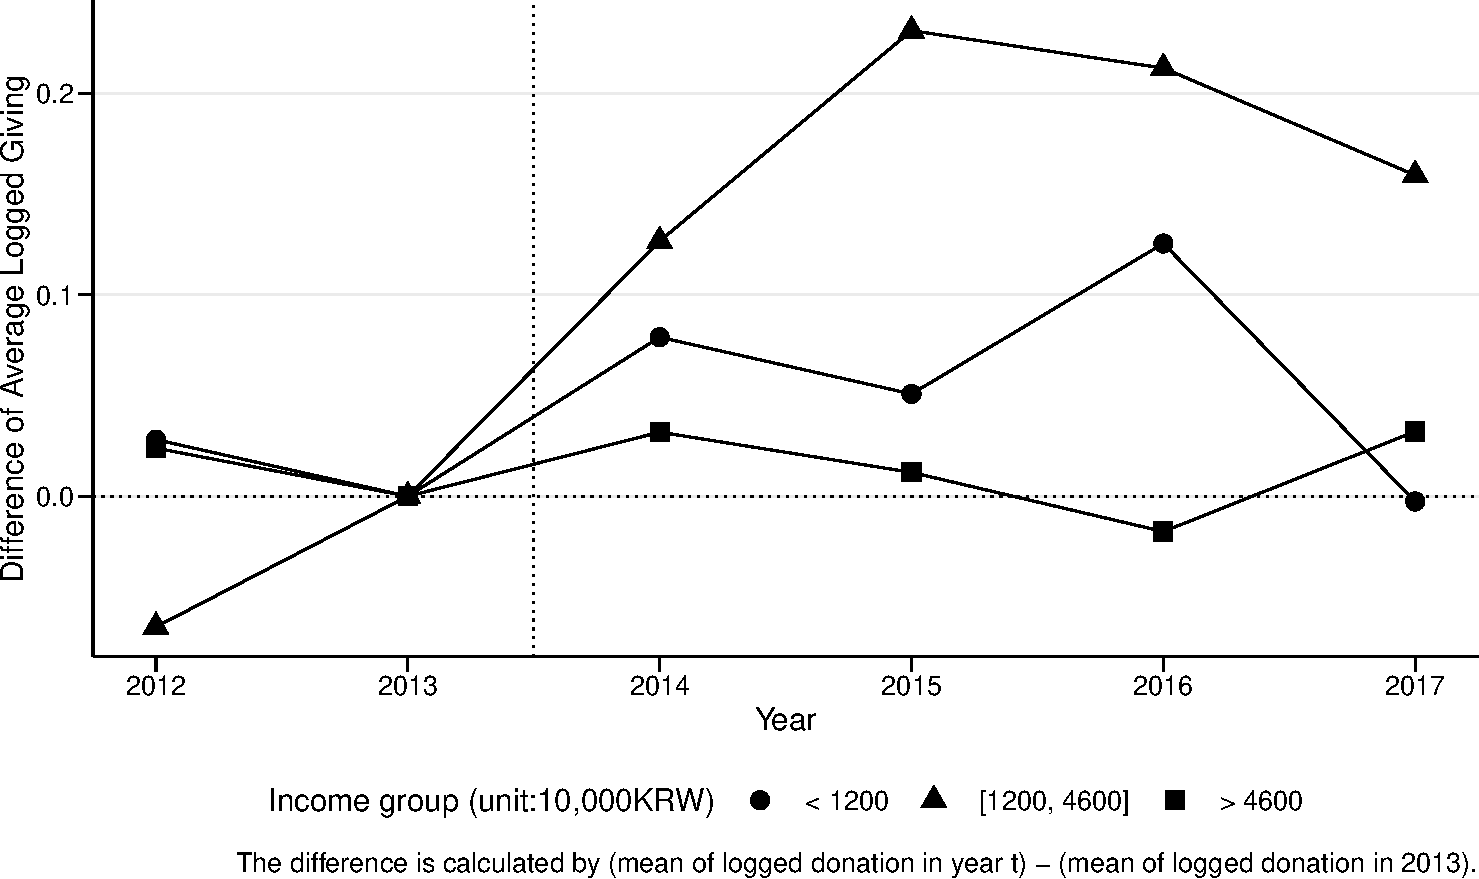
\includegraphics[width=0.7\linewidth,]{C:/Users/katoo/Desktop/NASTAB/paper/slide_files/figure-beamer/SummaryOutcomeIntensive-1} 

}

\caption{Average Logged Giving by Three Income Groups Conditional on Donors. Notes: We created three income groups, with the relative price of giving rising (circle), unchanged (triangle), and falling (square) between 2013 and 2014. The grup means are normalized to be one in 2013.}\label{fig:SummaryOutcomeIntensive}
\end{figure}
\end{frame}

\begin{frame}{Propotion of Donors by Income Groups (Extensive Margin)}
\protect\hypertarget{propotion-of-donors-by-income-groups-extensive-margin}{}
\begin{figure}[t]

{\centering 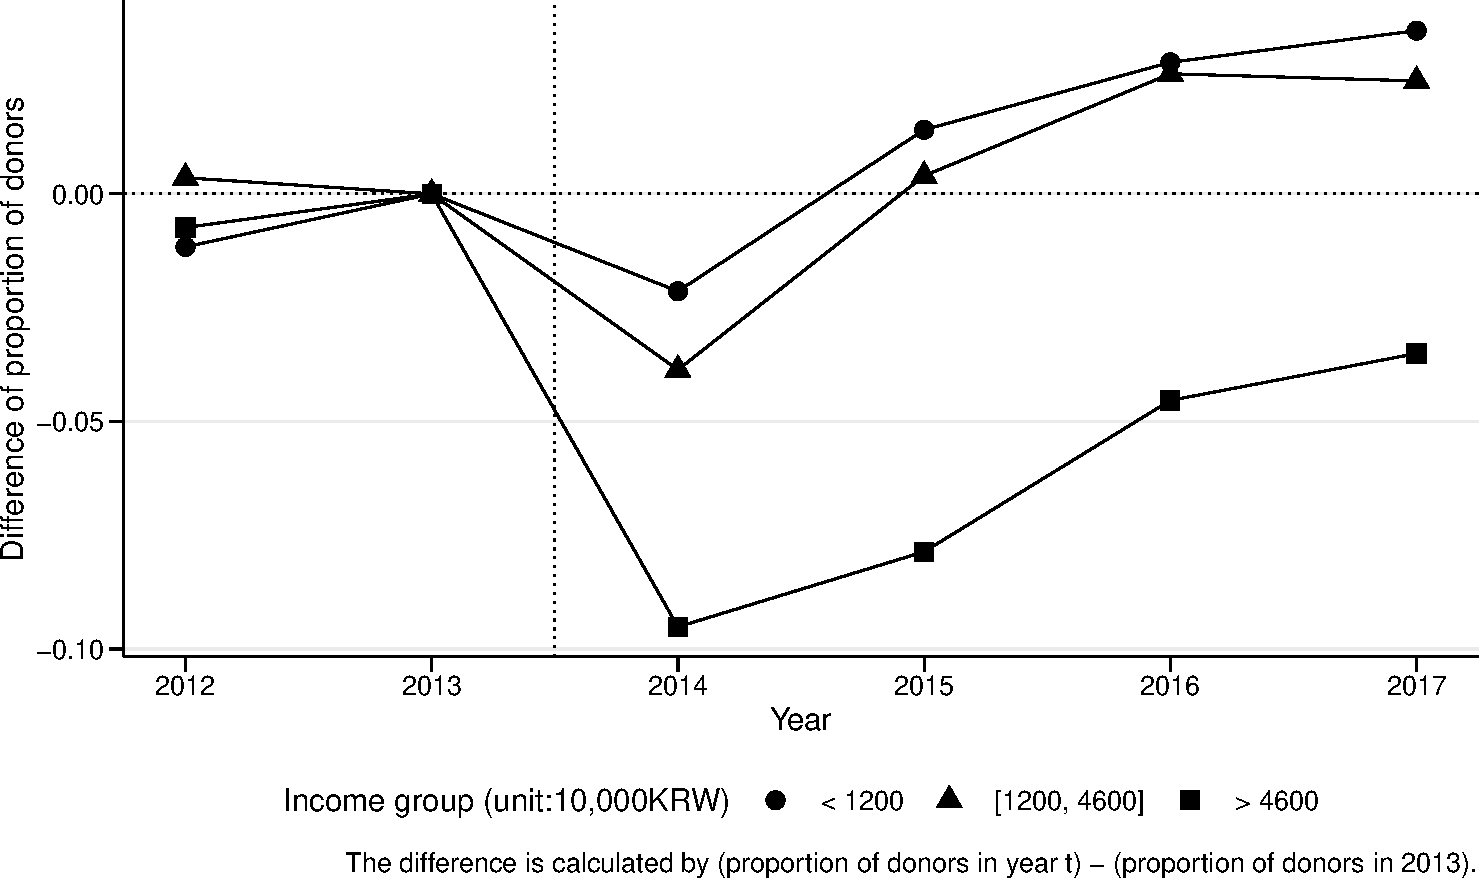
\includegraphics[width=0.7\linewidth,]{C:/Users/katoo/Desktop/NASTAB/paper/slide_files/figure-beamer/SummaryOutcome6-1} 

}

\caption{Proportion of Donors bn Three Income Groups. Notes: We created three income groups, with the relative price of giving rising (circle), unchanged (triangle), and falling (square) between 2013 and 2014. The grup means are normalized to be one in 2013.}\label{fig:SummaryOutcome6}
\end{figure}
\end{frame}

\begin{frame}{Distribution of Charitable Giving}
\protect\hypertarget{distribution-of-charitable-giving}{}
\begin{figure}[t]

{\centering 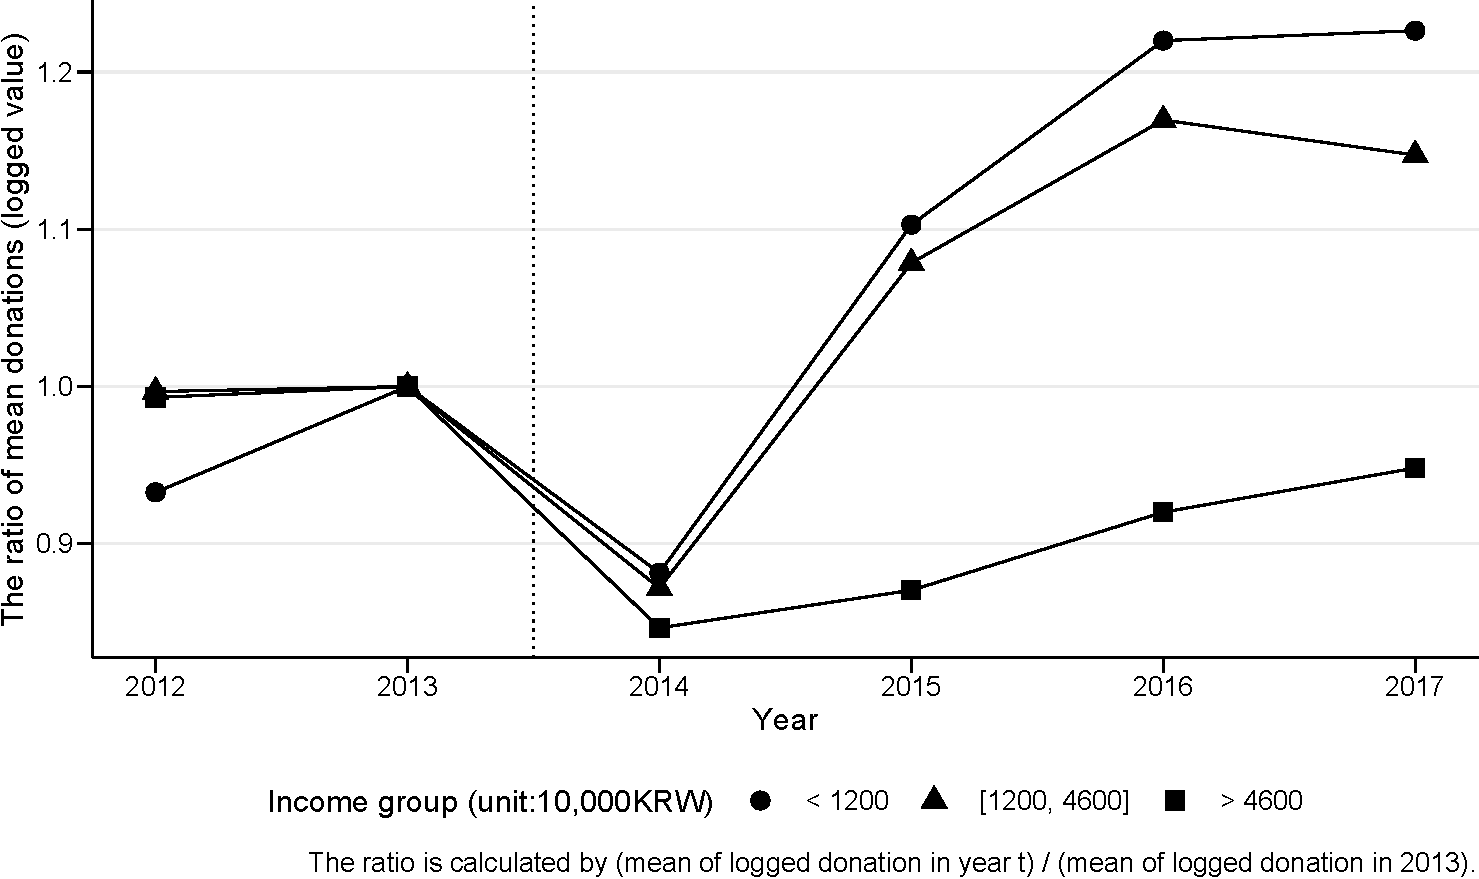
\includegraphics[width=0.85\linewidth,]{C:/Users/katoo/Desktop/NASTAB/paper/slide_files/figure-beamer/SummaryOutcome2-1} 

}

\caption{Distribution of Charitable Giving among Those Who Donated}\label{fig:SummaryOutcome2}
\end{figure}
\end{frame}

\begin{frame}{Proportion of Donors By Having Applied for Tax Relief}
\protect\hypertarget{proportion-of-donors-by-having-applied-for-tax-relief}{}
\begin{figure}[t]

{\centering 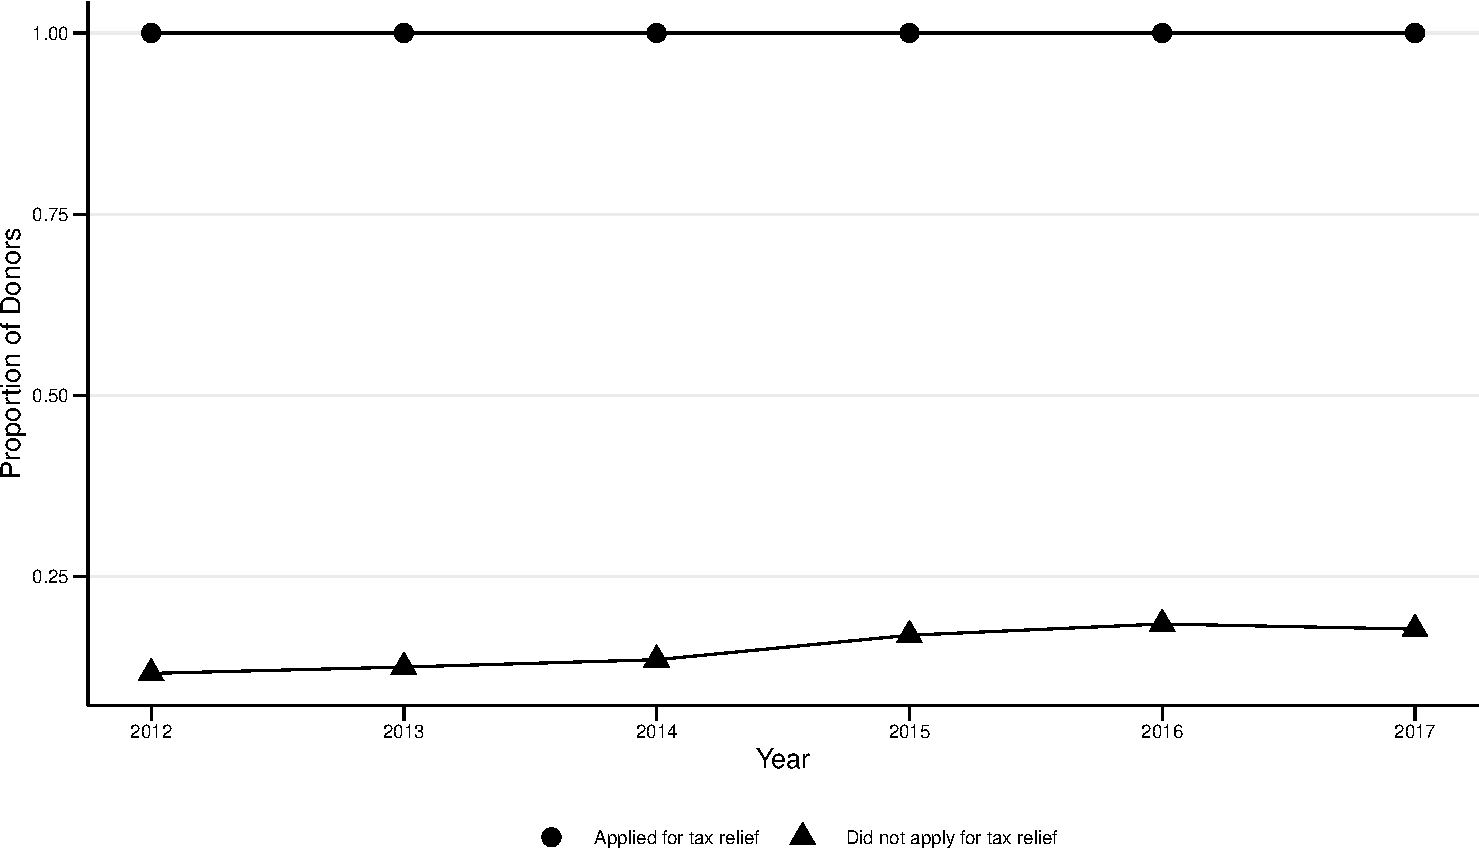
\includegraphics[width=0.85\linewidth,]{C:/Users/katoo/Desktop/NASTAB/paper/slide_files/figure-beamer/SummaryOutcome3-1} 

}

\caption{Proportion of Donors By Having Applied for Tax Relief}\label{fig:SummaryOutcome3}
\end{figure}
\end{frame}

\begin{frame}{Share of Tax Relief Grouped by Wage Earner or not}
\protect\hypertarget{share-of-tax-relief-grouped-by-wage-earner-or-not}{}
\begin{figure}[t]

{\centering 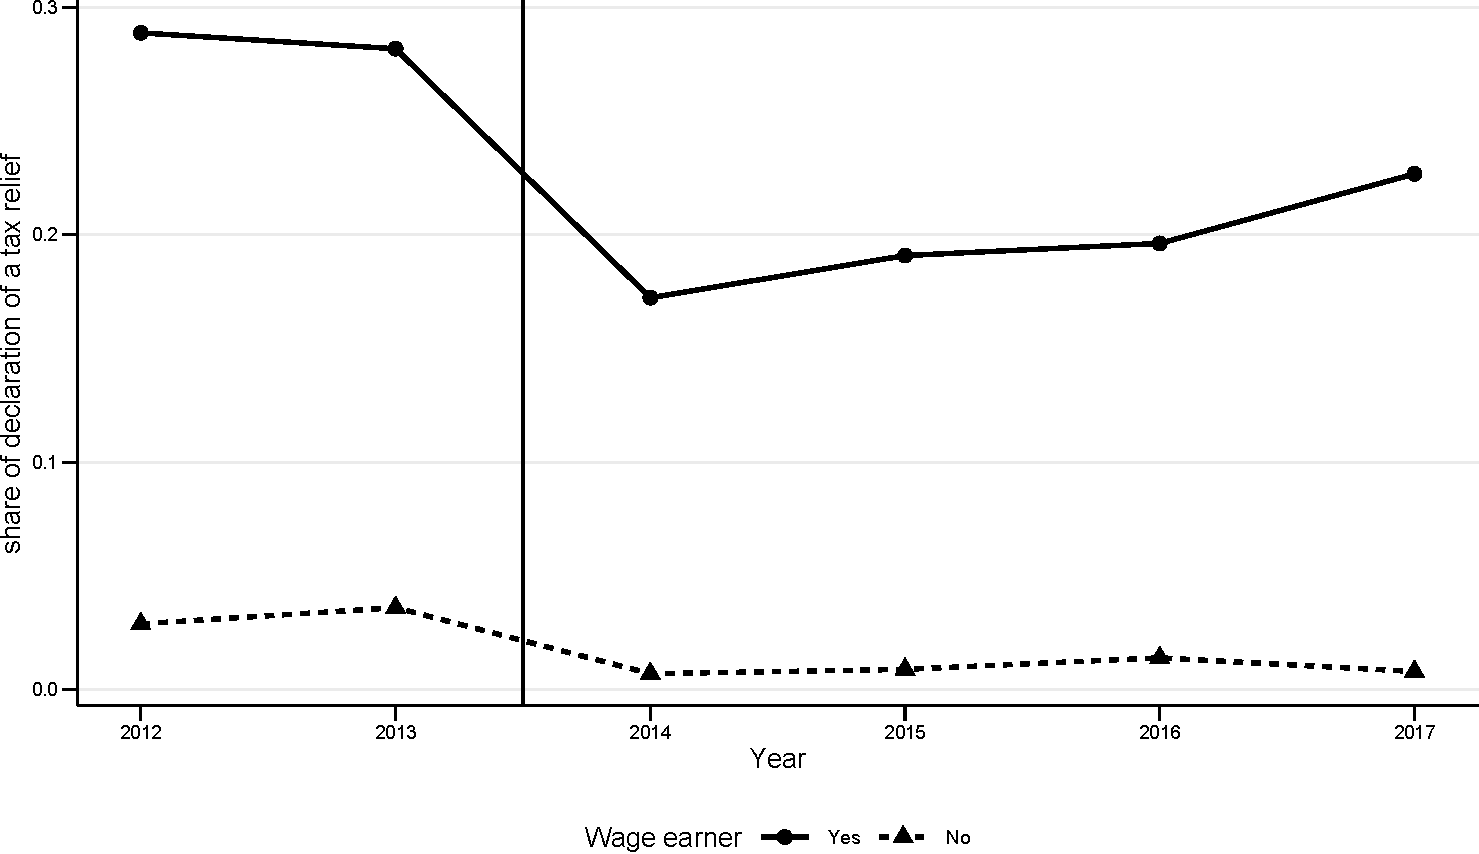
\includegraphics[width=0.7\linewidth,]{C:/Users/katoo/Desktop/NASTAB/paper/slide_files/figure-beamer/SummaryRelief-1} 

}

\caption{Share of Tax Relief. Notes: A solid line is the share of applying for tax relief among wage eaners. A dashed line is the share of applying for tax relief other than wage earners.}\label{fig:SummaryRelief}
\end{figure}
\end{frame}

\begin{frame}{Share of Tax Relief Grouped By Three Income Group}
\protect\hypertarget{share-of-tax-relief-grouped-by-three-income-group}{}
\begin{figure}[t]

{\centering 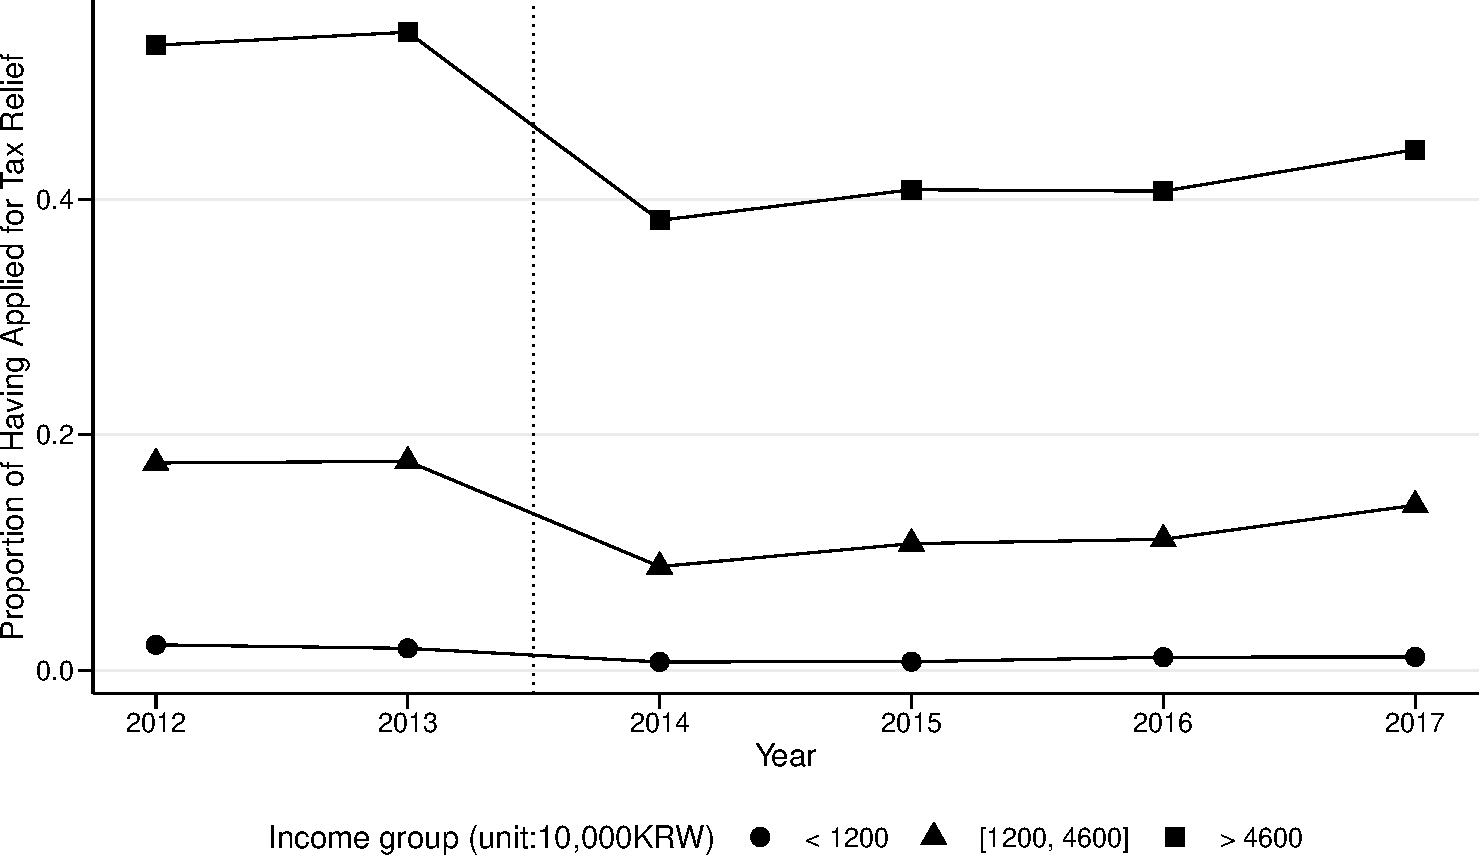
\includegraphics[width=0.85\linewidth,]{C:/Users/katoo/Desktop/NASTAB/paper/slide_files/figure-beamer/SummaryRelief2-1} 

}

\caption{Proportion of Having Applied for Tax Relief in Three Income Groups. Notes: We created three income groups, with the relative price of giving rising (circle), unchanged (triangle), and falling (square) between 2013 and 2014.}\label{fig:SummaryRelief2}
\end{figure}
\end{frame}

\hypertarget{first-stage-result-who-applied-for-tax-relief}{%
\section{First-Stage Result: Who Applied for Tax Relief?}\label{first-stage-result-who-applied-for-tax-relief}}

\hypertarget{estimating-conventional-price-elasticities}{%
\section{Estimating Conventional Price Elasticities}\label{estimating-conventional-price-elasticities}}

\hypertarget{control-function-approach}{%
\section{Control Function Approach}\label{control-function-approach}}

\hypertarget{welfare-implication}{%
\section{Welfare Implication}\label{welfare-implication}}

\hypertarget{conclusion}{%
\section{Conclusion}\label{conclusion}}

\hypertarget{references}{%
\section*{References}\label{references}}
\addcontentsline{toc}{section}{References}

\begin{frame}{References}
\hypertarget{refs}{}
\begin{CSLReferences}{1}{0}
\leavevmode\vadjust pre{\hypertarget{ref-Almunia2020}{}}%
Almunia, M., Guceri, I., Lockwood, B., Scharf, K., 2020. More giving or more givers? The effects of tax incentives on charitable donations in the UK. Journal of Public Economics 183. doi:\href{https://doi.org/10.1016/j.jpubeco.2019.104114}{10.1016/j.jpubeco.2019.104114}

\leavevmode\vadjust pre{\hypertarget{ref-Auten2002}{}}%
Auten, G.E., Sieg, H., Clotfelter, C.T., 2002. \href{http://www.jstor.org/stable/3083340}{Charitable giving, income, and taxes: An analysis of panel data}. American Economic Review 92, 371--382.

\leavevmode\vadjust pre{\hypertarget{ref-Fack2016}{}}%
Fack, G., Landais, C., 2016. The effect of tax enforcement on tax elasticities: Evidence from charitable contributions in france. Journal of Public Economics 133, 23--40. doi:\url{https://doi.org/10.1016/j.jpubeco.2015.10.004}

\leavevmode\vadjust pre{\hypertarget{ref-Gillitzer2018}{}}%
Gillitzer, C., Skov, P.E., 2018. {The use of third-party information reporting for tax deductions: evidence and implications from charitable deductions in Denmark}. Oxford Economic Papers 70, 892--916. doi:\href{https://doi.org/10.1093/oep/gpx055}{10.1093/oep/gpx055}

\leavevmode\vadjust pre{\hypertarget{ref-Saez2004}{}}%
Saez, E., 2004. The optimal treatment of tax expenditures. Journal of Public Economics 88, 2657--2684. doi:\href{https://doi.org/10.1016/j.jpubeco.2003.09.004}{10.1016/j.jpubeco.2003.09.004}

\end{CSLReferences}
\end{frame}

\end{document}
